\documentclass{ctexbeamer} %

% 载入TikZ宏包
\usepackage{tikz}
% 载入TikZ库
\usetikzlibrary{
  arrows.meta,      % 箭头形状
  shapes.geometric, % 几何形状
  chains,           % 链式布局
  calc,             % 坐标计算
}

% 为使用外部节点,需要为TikZ指定'remember picture'样式
% 为了方便在导言区进行全局设置
\tikzstyle{every picture}+=[remember picture]
% 将数学公式统一设置为displaystyle样式.
\everymath{\displaystyle}

% 示例图等
\usepackage{mwe}

\begin{document}
\begin{frame}{彩色公式}{标记公式}
  % 定义TikZ样式                
  \tikzstyle{na} = [baseline=-.5ex]
                
  \begin{itemize}
  \item A \tikz[baseline]{\node[blue,anchor=base] (t1) {bilinear
        model};} for classification is a \tikz[baseline]{\node[blue,anchor=base] (t2) {four-tuple};}    
  \end{itemize}
                
  % 在公式中使用TikZ节点
  % 注意:为了对齐,需要调整节点的baseline
  \begin{equation*}
    \mathcal{B} =(
    \tikz[baseline]{
      \node[fill=green!20,anchor=base] (m1)
      {$f_{A},f_{B}$};
    },
    \tikz[baseline]{
      \node[fill=blue!20, anchor=base] (m2)
      {$\mathcal{P}$};
    },
    \tikz[baseline]{
      \node[fill=red!20, anchor=base] (m3)
      {$\mathcal{C}$};
    }
    )
  \end{equation*}

  \begin{center}
    
\begin{tikzpicture}
      \node[fill=green!30] (n1) at (0,0) {feature extractor};
      \node[fill=blue!30, right =0.25 of n1] (n2) {pooling};
      \node[fill=red!30, right =0.25 of n2] (n3) {classification};
    \end{tikzpicture}
  \end{center}

  \begin{center}
    $f:\mathcal{L}\times \mathcal{I}\rightarrow
        R^{c\times D}$  e.g., SIFT is $\mathcal{R}^{1\times 128}$
  \end{center}

  
\begin{tikzpicture}
    \node[fill=gray!20](nn1) at (0,0) {image};
    \node[fill=green!40, right = 2 of nn1](nn2) {local features};
    \draw[-{Stealth[scale=1.0]}, thick] (nn1.east)--(nn2.west);
  \end{tikzpicture}

  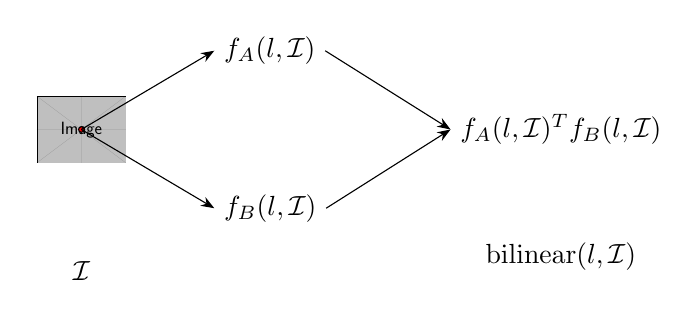
\begin{tikzpicture}
    \node(i1) at (0,0) {\includegraphics[scale=0.1]{example-image}};
    \node[right= of i1, yshift=1.0cm](i2) {$f_{A}(l, \mathcal{I})$};
    \node[right= of i1, yshift=-1.0cm](i3) {$f_{B}(l, \mathcal{I})$};
    \node[right=4 of i1](i4) {$f_{A}(l, \mathcal{I})^{T}f_{B}(l, \mathcal{I})$};
    \node[below= of i1](i5) {$\mathcal{I}$};
    \node[below= of i4](i6) {bilinear$(l,\mathcal{I})$};
    \draw[fill=red](i1.center) circle(1pt);
    \draw[-{Stealth[scale=1.0]}] (i1.center)--(i2.west);
    \draw[-{Stealth[scale=1.0]}] (i1.center)--(i3.west);
    \draw[-{Stealth[scale=1.0]}] (i2.east)--(i4.west);
    \draw[-{Stealth[scale=1.0]}] (i3.east)--(i4.west);
  \end{tikzpicture}

  % 绘制文本与公式中标记点连线
  \begin{tikzpicture}[overlay]
    \draw[-{Stealth[scale=1.0]}] (n1.north)--(m1.south);
    \draw[-{Stealth[scale=1.0]}] (n2.north)--(m2.south);
    \draw[-{Stealth[scale=1.0]}] (n3.north)--(m3.south);
  \end{tikzpicture}    
\end{frame}
\end{document}
%%% Local Variables:
%%% mode: latex
%%% TeX-master: t
%%% End:
